%%%%%%%%%%%%%%%%%%%%%%%%%%%%%%%%%%%%%%%%%
% Beamer Presentation
% LaTeX Template
% Version 1.0 (10/11/12)
%
% This template has been downloaded from:
% http://www.LaTeXTemplates.com
%
% License:
% CC BY-NC-SA 3.0 (http://creativecommons.org/licenses/by-nc-sa/3.0/)
%
%%%%%%%%%%%%%%%%%%%%%%%%%%%%%%%%%%%%%%%%%

%----------------------------------------------------------------------------------------
%	PACKAGES AND THEMES
%----------------------------------------------------------------------------------------

\documentclass{beamer}


\usepackage{epsf}

\usepackage{float}
\usepackage{setspace}


\usepackage{epsfig}
\usepackage{caption}
\usepackage{subfig}
\usepackage{graphicx}

\mode<presentation> {

% The Beamer class comes with a number of default slide themes
% which change the colors and layouts of slides. Below this is a list
% of all the themes, uncomment each in turn to see what they look like.

%\usetheme{default}
%\usetheme{AnnArbor}
%\usetheme{Antibes}
%\usetheme{Bergen}
%\usetheme{Berkeley}
%\usetheme{Berlin}
%\usetheme{Boadilla}
%\usetheme{CambridgeUS}
%\usetheme{Copenhagen}
%\usetheme{Darmstadt}
%\usetheme{Dresden}
%\usetheme{Frankfurt}
%\usetheme{Goettingen}
%\usetheme{Hannover}
%\usetheme{Ilmenau}
%\usetheme{JuanLesPins}
%\usetheme{Luebeck}
\usetheme{Madrid}
%\usetheme{Malmoe}
%\usetheme{Marburg}
%\usetheme{Montpellier}
%\usetheme{PaloAlto}
%\usetheme{Pittsburgh}
%\usetheme{Rochester}
%\usetheme{Singapore}
%\usetheme{Szeged}
%\usetheme{Warsaw}

% As well as themes, the Beamer class has a number of color themes
% for any slide theme. Uncomment each of these in turn to see how it
% changes the colors of your current slide theme.

%\usecolortheme{albatross}
%\usecolortheme{beaver}
%\usecolortheme{beetle}
%\usecolortheme{crane}
%\usecolortheme{dolphin}
%\usecolortheme{dove}
%\usecolortheme{fly}
%\usecolortheme{lily}
%\usecolortheme{orchid}
%\usecolortheme{rose}
%\usecolortheme{seagull}
%\usecolortheme{seahorse}
%\usecolortheme{whale}
%\usecolortheme{wolverine}

%\setbeamertemplate{footline} % To remove the footer line in all slides uncomment this line
%\setbeamertemplate{footline}[page number] % To replace the footer line in all slides with a simple slide count uncomment this line

%\setbeamertemplate{navigation symbols}{} % To remove the navigation symbols from the bottom of all slides uncomment this line
}

\usepackage{graphicx} % Allows including images
\usepackage{booktabs} % Allows the use of \toprule, \midrule and \bottomrule in tables

%----------------------------------------------------------------------------------------
%	TITLE PAGE
%----------------------------------------------------------------------------------------

\title[TMTC FE]{Telemetry / Telecommand Frontend} % The short title appears at the bottom of every slide, the full title is only on the title page

\author{Anoop R Santhosh} % Your name
\institute[IITM] % Your institution as it will appear on the bottom of every slide, may be shorthand to save space
{
Indian Institute of Technology, Madras \\ % Your institution for the title page
\medskip
\textit{anoop@cse.iitm.ac.in} % Your email address
}
\date{\today} % Date, can be changed to a custom date

\begin{document}

\begin{frame}
\titlepage % Print the title page as the first slide
\end{frame}

\begin{frame}
\frametitle{Overview} % Table of contents slide, comment this block out to remove it
\tableofcontents % Throughout your presentation, if you choose to use \section{} and \subsection{} commands, these will automatically be printed on this slide as an overview of your presentation
\end{frame}

%----------------------------------------------------------------------------------------
%	PRESENTATION SLIDES
%----------------------------------------------------------------------------------------

%------------------------------------------------
\section{Introduction} % Sections can be created in order to organize your presentation into discrete blocks, all sections and subsections are automatically printed in the table of contents as an overview of the talk
%------------------------------------------------

\subsection{IITMSAT} % A subsection can be created just before a set of slides with a common theme to further break down your presentation into chunks

\begin{frame}
\frametitle{IITMSAT - A Brief Introduction}
\pause
\begin{itemize}
\item Student initiated satellite project at IIT Madras.
\pause
\item Low orbit nano satellite (Mass 15kg).
\pause
\item Onboard high energy particle detector to measure changes in flux of charged particles in ionosphere.
\pause
\item Aims to study the correlation between earth based phenomenon and changes in flux.
\pause
\item Mission Life Time : greater than 1 year

\end{itemize}
\end{frame}

%------------------------------------------------

\begin{frame}
\frametitle{IITMSAT - A Brief Introduction}
\pause
\begin{itemize}
\item Various subsystems, both hardware and software involved.
\pause
\item The focus here is on Ground Station  software, especially a module within it, TMTC Frontend.
\end{itemize}
\end{frame}

%------------------------------------------------
\subsection{Ground Station Software}
\begin{frame}
\frametitle{Ground Station Software}
\pause
\begin{itemize}
\item Handles Operations of the satellite from ground.
\pause
\item Processes the information transmitted by satellite.
\pause
\item Three major components 
\begin{itemize}
\item User Interface
\item Mission Control System
\item TMTC Frontend
\end{itemize}
\end{itemize}

\end{frame}

%------------------------------------------------

\begin{frame}
\frametitle{Ground Station Block Diagram}
\begin{figure}
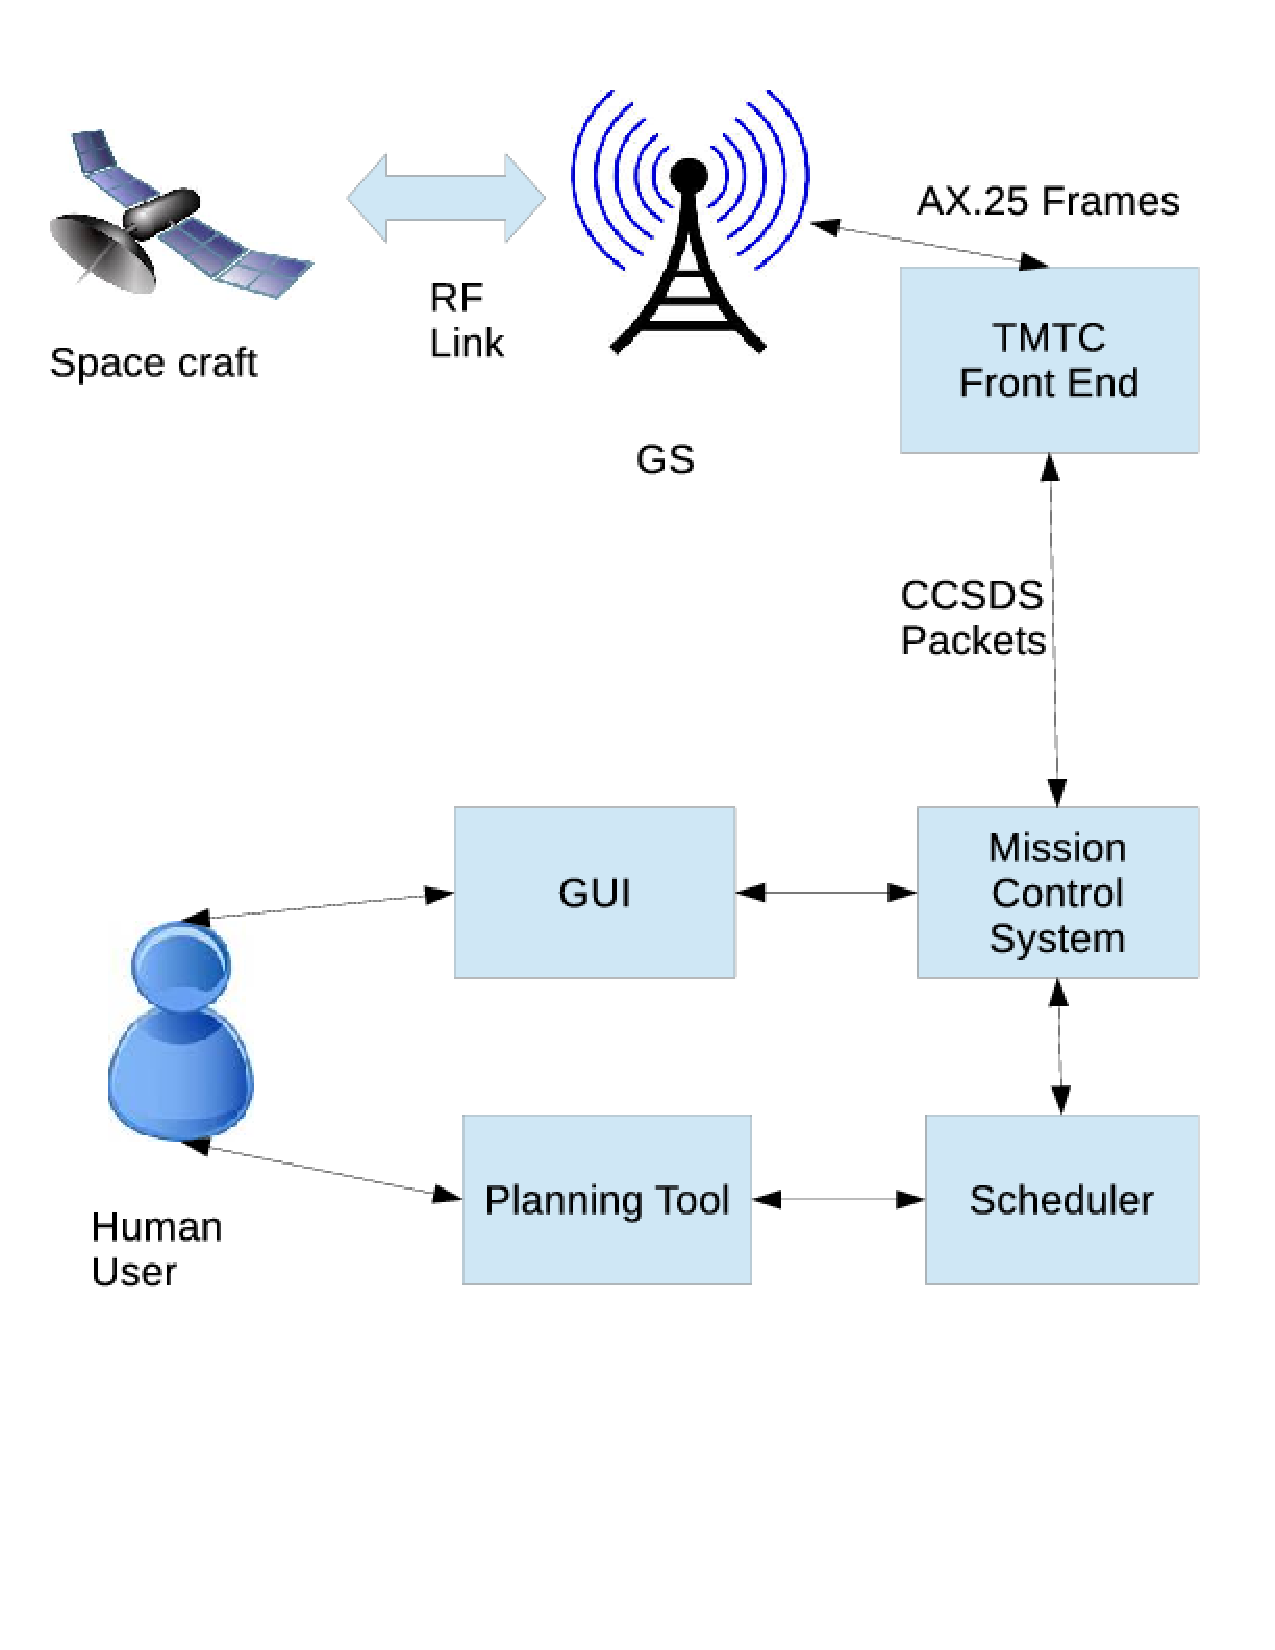
\includegraphics[scale = 0.3 ]{gs.pdf}
\caption{Block Diagram}
\label{fig1:gs}
\end{figure}

\end{frame}


%------------------------------------------------
\section{Telemetry/ Telecommand Frontend}
%------------------------------------------------

\subsection{TMTC Frontend}
\begin{frame}
\frametitle{TMTC Frontend - Problem Statement}
\pause 
\begin{itemize}
\item Link layer between MCS and satellite.
\pause
\item Implement a robust TMTC Frontend.
\pause
\item The main functionalities of TMTC Frontend are 
\begin{itemize}
\item \textbf{Uplink}
\begin{itemize}
\item Encoding CCSDS packets (telecommand) to AX.25 frame.
\item Archive AX.25 telecommand frames.
\item Flow Control (resending, counters, acknowledgments etc ).
\end{itemize}
\item \textbf{Downlink}
\begin{itemize}
\item Decode AX.25 frame (telemetry) and reassemble the application data to
obtain CCSDS packets.
\item Archive raw AX.25 telemetry frames.

\end{itemize}

\item \textbf{Replay}
\begin{itemize}
\item Provide functionality to replay archived raw AX.25 telemetry frames.
\end{itemize}
\end{itemize}
\end{itemize}
\end{frame}

\begin{frame}
\frametitle{TMTC Frontend - Block Diagram}
\begin{figure}
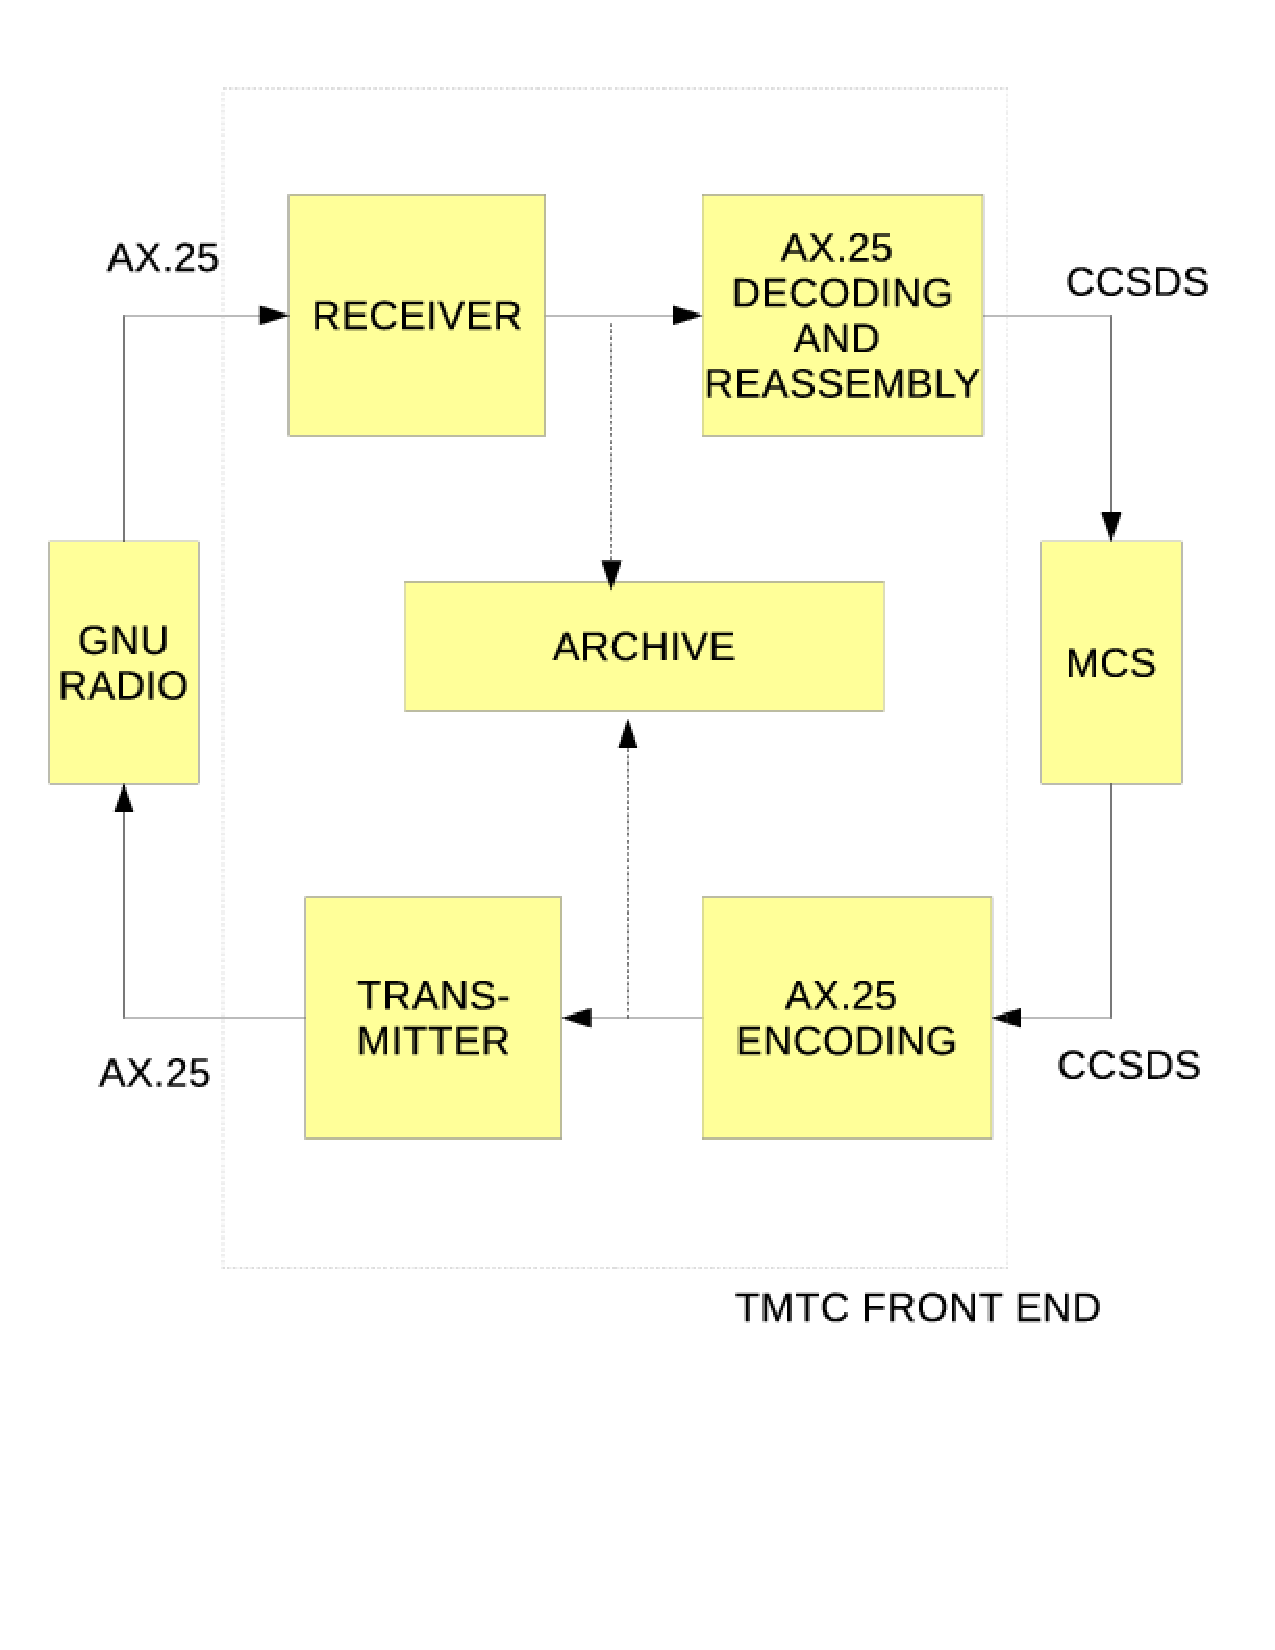
\includegraphics[scale = 0.3 ]{tmtc.pdf}
\caption{Block Diagram}
\label{fig1:tmtc}
\end{figure}
\end{frame}

\begin{frame}
\frametitle{Motivation}
\begin{itemize}
\item Communication link may not be very reliable.
\item Limited time of communication.
\item Need to transfer data reliably in that time.
\item A robust link layer is essential for that.
\end{itemize}
\end{frame}

\begin{frame}
\frametitle{Related Work}
\begin{itemize}
\item SwissCube Ground Station Software.
\item Our design is loosely based on it.

\end{itemize}
\end{frame}
\begin{frame}
\frametitle{Main Contribution}
\begin{itemize}


\item Implementation of modified AX.25 protocol encoding/decoding.
\item Modification of TC Transmitter.
\item Reassembly unit.
\item Implementation of entire module in general.
\end{itemize}
\end{frame}
\section{Communication Protocol}
\subsection{Modified AX.25 Protocol}
\begin{frame}
\frametitle{Modified AX.25 Frame}
\begin{figure}
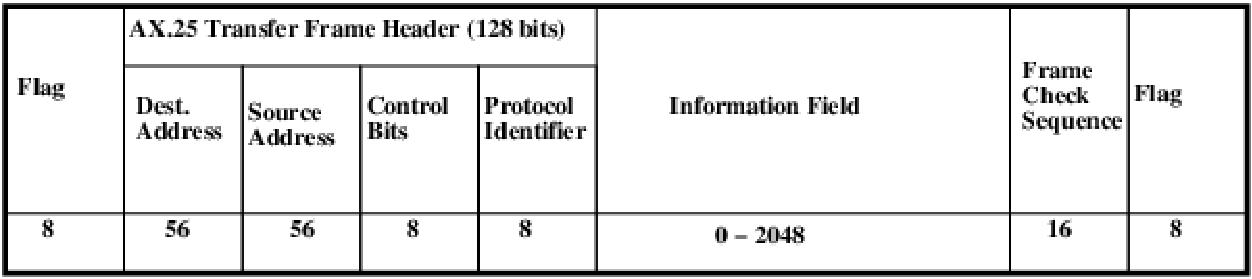
\includegraphics[scale = 0.5 ]{ax25main.pdf}
\caption{Frame Structure. Adapted from [1].}
\label{fig1:ax25main}
\end{figure}
\begin{itemize}
\item In case of telecommand frames, first byte of information field is set as counter.
\end{itemize}
\end{frame}

\begin{frame}
\frametitle{Telemetry Information Field Usage}
\begin{figure}
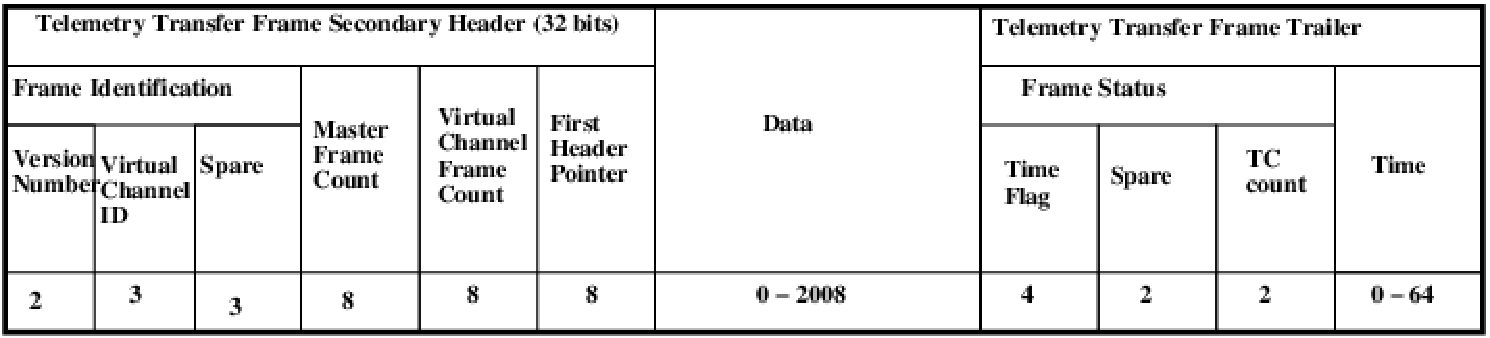
\includegraphics[scale = 0.35 ]{ax25telemetry.pdf}
\caption{Frame Structure}
\label{fig1:ax25telemetry}
\end{figure}
\begin{itemize}
\item Virtual Channels.
\item Large Data Transfer.
\end{itemize}
\end{frame}


\section{Design}

\begin{frame}
\frametitle{Design of TMTC Frontend}
TMTC Frontend consists of four major sub modules :
\begin{itemize}
\item AX.25 Packet Encoding/ Decoding.
\item TC Transmitter.
\item TM Receiver.
\item Replay Controller.
\end{itemize}
\end{frame}
\subsection{TC Transmitter}
\begin{frame}
\frametitle{Limitations of Swiss cube TC Transmitter Design }
\begin{itemize}
\item It can support only 4 outstanding packets.
\item Packets are transmitted one at a time.
\item Transmission of packets are manually controlled by the user through MCS.
\item There was no option of resending at TMTC Frontend layer.
\item In the event of packet drop, the information is carried back to the application
level, where a human user decides to resend the packet again.

\end{itemize}
\end{frame}

\begin{frame}
\frametitle{Modified Design}
The important features of the modified design are :
\begin{itemize}
 \item Packets are transmitted when transmitter is on and positive beacon signal is
received.
\item  All the packets in the ready queue are dispatched at the same time one after
another. The number of packets is expected to be in the order of 10, which is
way less than the 256 outstanding packets allowed.

\item  Transmitter is half duplex. So we are not implementing an explicit timeout.
Acknowledgment for a frame sent in a transmitter period is expected to
come in the immediate next receiver period.
\item If acknowledgement is not received in the immediate next reception, packet
is resent.A packet will be resent a fixed number of times, after which packet
drop will be announced to MCS.

\end{itemize}
\end{frame}

\begin{frame}
\frametitle{States}
There are three states :
\begin{itemize}
\item READY .
\item WAIT\_FOR\_ACK .
\item WAIT\_FOR\_TRANS . 
\end{itemize}


\end{frame}

\begin{frame}
\frametitle{External Triggers}
The external triggers are :
\begin{itemize}
\item Transmitter ON : Indicates switch to transmission mode.
\item Transmitter OFF : Indicates switch to reception mode.
\item Positive Beacon : Indicates that satellite is in field of view and ready for reception.
\item Ack received : Indicates the reception of acknowledgement packet by receiver.

\end{itemize}
\end{frame}

\begin{frame}
\frametitle{State Diagram}
\begin{figure}
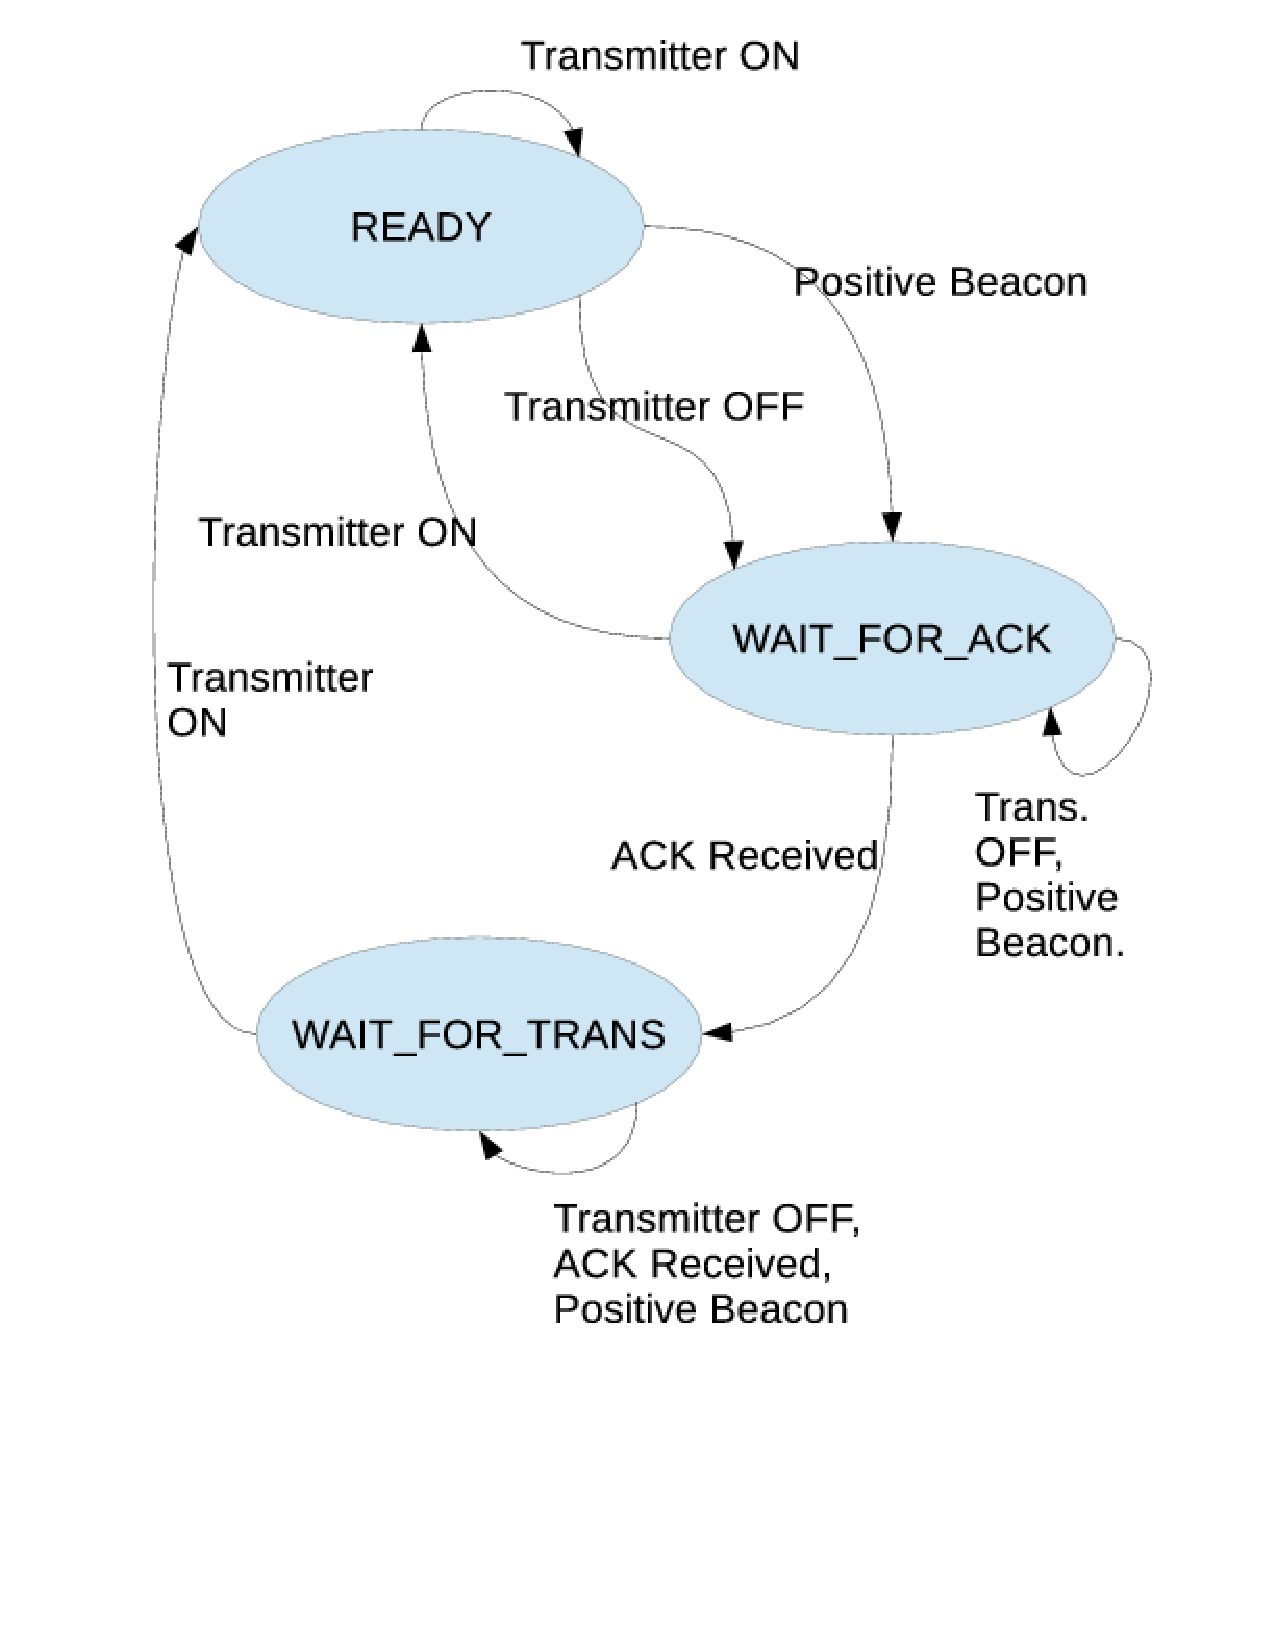
\includegraphics[scale = 0.35 ]{state.pdf}
\caption{State Diagram}
\label{fig1:state}
\end{figure}
\end{frame}

\subsection{TM Receiver}
\begin{frame}
\frametitle{TM Receiver Design}
Processing steps after reception of an AX.25 telemetry frame in that order is as follows. 
\begin{enumerate}
\item Receive AX.25 frame.
\item CRC check to detect frame bit errors.
\item Check the GS and Satellite SSID and Callsign.
\item If the frame is an acknowledgement frame, trigger Acknowledgment received of receiver.
\item Otherwise Archive the raw frame in database .
\item Forward the frame to appropriate virtual channel.
\item Transfer the frame to reassembly unit of the virtual channel.
\item After a CCSDS packet is completely reassembled, forward it to the MCS on appropriate port or channel. 
\end{enumerate}

\end{frame}

\subsection{Replay Controller}
\begin{frame}
\frametitle{Replay Controller}
\begin{figure}
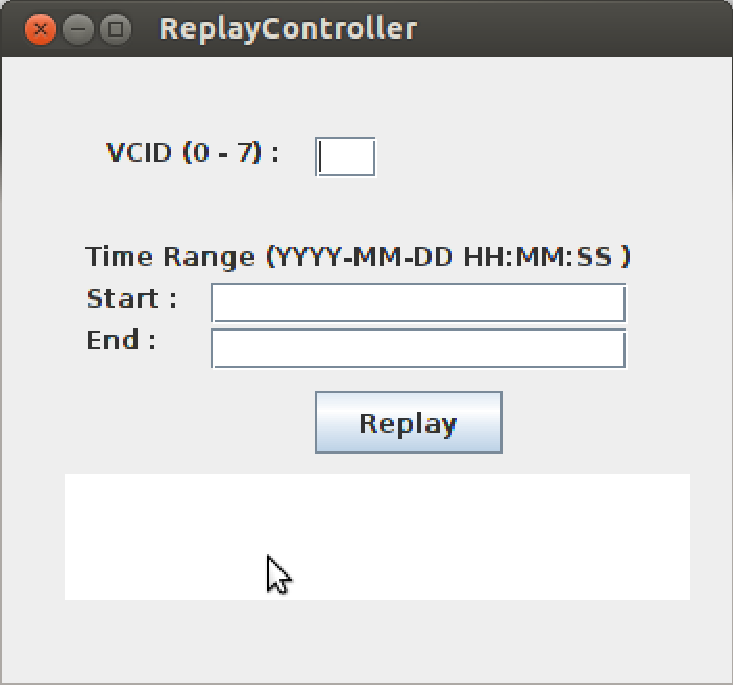
\includegraphics[scale = 0.4 ]{replay.pdf}
\caption{User Interface}
\label{fig1:replay}
\end{figure}
\end{frame}

\section{Implementation}
\begin{frame}
\frametitle{Implementation Details - Development environment}
\begin{itemize}
\item \textbf{Development Language : } Java 1.6.0
\item \textbf{Development Environment : } Eclipse IDE
\item \textbf{Database server : } MySQL 5.5.35
\item \textbf{Operating System : }Ubuntu 12.04
\end{itemize} 
\end{frame}

\begin{frame}
\frametitle{Important Modules}
The important modules with TMTC Frontend are :
\begin{itemize}
\item AX.25 encoding/decoding.
\item TC Transmitter.
\item TM Receiver.
\item Replay Controller.
\item Archiving Frames.
\item Reassembly Unit.
\end{itemize}
\end{frame}

\section{Testing}
\begin{frame}
\frametitle{Testing Details}
\begin{itemize}
\item Different units were tested individually by writing various test cases.
\item Simulators not available for MCS or SDR.
\item Approximate conditions were simulated and various features like frame drop, resend etc were tested.
\end{itemize}
\end{frame}

\section{Summary}
\begin{frame}
\frametitle{Summary}
\begin{itemize}
\item TMTC Frontend implemented in Java taking care of current expected scenario.
\item Modified the design to suit IITMSAT requirements.
\item Limited testing was done based on available details.
\item Integration with other modules and rigorous testing after integration are left.
\end{itemize}
\end{frame}

\section{Bibliography}
\begin{frame}
\frametitle{Bibliography}
\begin{thebibliography}{50}
\bibitem{ax25} Beech, William A., Douglas E. Nielsen, and Jack Taylor. AX.25 Link Access Protocol for Amateur Packet Radio , 2.2nd ed. Tucson, Arizona: Tucson Amateur Packet Radio Corporation,July 1998.
\bibitem{ccsds102}Packet Telemetry. Recommendation for Space Data System Standards, CCSDS
102.0-B-5. Blue Book. Issue 5. Washington, D.C.: CCSDS, November 2000.
\bibitem{ecss}Ground systems and operations — Telemetry and telecommand packet utilization,ECSS--E--70--41A.
Noordwijk,The Netherlands.:ESA Publications Division,January 2003.

\bibitem{swisscube1}Yann Voumard. TM/TC Front End Phase C,S3-C-S E-1-3-TMTC Front End Report
.Issue 1.Noordwijk,The Netherlands,ESA,June 2008.


\bibitem{swisscube2}Florian George and Benoit Cosandier. SwissCube Ground Segment Phase B,S3-B-S E-1-5-Ground Segment.Issue 1.Noordwijk,The Netherlands,ESA ,June 2008.


\end{thebibliography}
\end{frame}
%------------------------------------------------
%------------------------------------------------


%------------------------------------------------



%------------------------------------------------



%------------------------------------------------


%------------------------------------------------



%----------------------------------------------------------------------------------------

\end{document} 